\chapter{Sistemi Informativi e Privacy}

\section{Sistemi Informativi}

\qs{}{Che cos'è un sistema informativo?}

\dfn{Sistema Informativo}{
  Un sistema informativo è un sistema formale, sociotecnico e orgazzativo per collezionare, processare, raccogliere e distribuire informazioni usate da organizzazioni.
}

\cor{Sistema Informativo Computazionale}{
  Un sistema informativo computazionale è un sistema composto da persone e computer ce processano o interpretano informazioni.
}

\paragraph{Lo scopo di un sistema informativo è quello di supportare:}

\begin{itemize}
  \item Le attività (automazione). 
  \item Le decisioni prese dagli alti ranghi di organizzazioni (analisi, controllo, coordinazione, statistica).
\end{itemize}

\paragraph{I sistemi informativi funzionano grazie agli scambi di dati e informazioni:}

\begin{itemize}
  \item Dati modellati come insiemi di processi interconnessi dove l'output di un processo è l'input di un altro processo. 
  \item I dati appartengono a diverse entità: 
    \begin{itemize}
      \item Impiegati. 
      \item Clienti.
      \item Fornitori.
    \end{itemize}
  \item Differenti tipi di dati:
    \begin{itemize}
      \item Identificativi personali. 
      \item Emails.
      \item Dati di processi, transazioni, etc.
    \end{itemize}
\end{itemize}

\paragraph{Un sistema informativo, per essere conforme al GDPR, deve assicurare:}

\begin{itemize}
  \item \fancyglitter{Autorizzazione basata su attributi:} meccanismi per accedere a tutti i dati, sotto determinate circostanze.
  \item \fancyglitter{Anonimizzazione} e \fancyglitter{Pseudoanonimizzazione} dei dati: meccanismi per garantire l'anonimato o lo pseudoanonimato.
  \item \fancyglitter{Tracciabilità:} un registro di chi ha creato, modificato o cancellato informazioni, quando e per quale scopo. 
  \item \fancyglitter{Cancellazione dei dati:} meccanismi per il diritto all'oblio.
\end{itemize}

\subsection{Tecniche di Controllo degli Accessi}

\dfn{Controllo degli Accessi}{
  Si restringe l'accesso alle risorse computazionali, specialmente in sistemi multi-utente.
}

\nt{I requisiti di privacy e sicurezza devono essere mantenuti nel sistema in modo efficiente. Tuttavia in situazioni di emergenza si possono fare delle eccezioni (e.g. in un ospedale con un paziente in pericolo di vita).}

\cor{Role Based Access Control (RBAC)}{
  Formalizzato da NIST nel 1992. Si gestisce l'accesso in base al ruolo invece che a un identificatore. Il ruolo fornisce un livello di astrazione (come collezione di permessi). Ogni ruolo può essere assegnato a un numero arbitrario di utenti.
}

\qs{}{Come funziona RBAC (fig: \ref{fig:rbac})?}

\begin{itemize}
  \item Gli \fancyglitter{amministratori} assegnano permessi a ogni ruolo. 
  \item I ruoli possono essere assegnati a utenti individuali (e ogni utente può avere più ruoli). 
  \item Gli amministratori possono aggiornare i ruoli aggiungendoli o rimuovendoli da determinati utenti.
\end{itemize}

\begin{figure}[h]
    \centering
    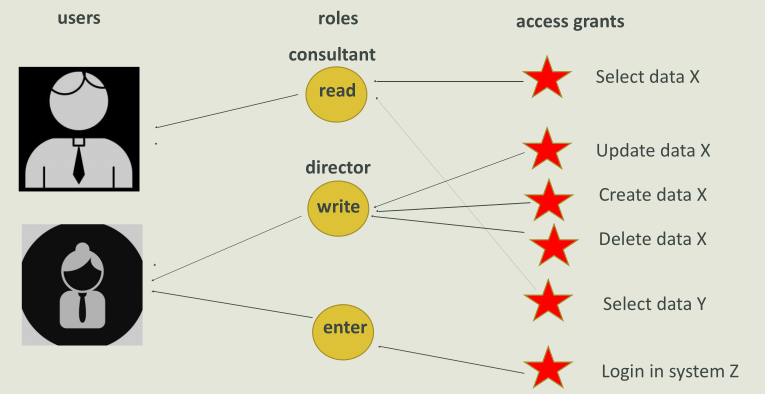
\includegraphics[scale=0.5]{02P/RBAC.png}
    \caption{RBAC.}
    \label{fig:rbac}

  \end{figure}

\paragraph{Limiti di RBAC:}

\begin{itemize}
  \item Non fornisce un meccanismo flessibili per cui i clienti possano esprimere dei loro requisiti. 
  \item Non cattura lo scopo per cui i dati vengono rilasciati. 
  \item Per cui RBAC si evolve in Attribute Base Access Control (ABAC).
\end{itemize}

\paragraph{Aggiungendo contesto, le decisioni autorizzative possono essere basate su:}

\begin{itemize}
  \item Ruolo. 
  \item Persone od oggetti collegati all'utente. 
  \item Di che cosa si ha bisogno. 
  \item Dove l'utente vuole accedere. 
  \item Quando l'utente vuole accedere. 
  \item Com'è l'utente vuole accedere a quelle informazioni.
\end{itemize}

\cor{Attribute Based Access Control (ABAC)}{
  Definendo un contesto si possono aggiungere adeguate politiche di accesso che definiscono in maniera dichiarativa come debba avvenire l'accesso.
}

\nt{Conoscere il ruolo di un utente non è abbastanza per assicurare la sicurezza. Si richiede il contesto e le relazioni tra le varie entità presenti nel sistema.}

\paragraph{Caratteristiche di ABAC(fig: \ref{fig:abac}):}

\begin{itemize}
  \item Adotta un approccio \fancyglitter{policy driven}. 
  \item Usa gli attributi \fancyglitter{soggetto}, \fancyglitter{oggetto} e \fancyglitter{ambiente}. 
  \item Rimuove la necessità di dover essere registrati in un sistema per essere in grado di accedere a risorse condivise.
  \item Utilizza un \fancyglitter{authorization engine} (fig: \ref{fig:auth}).
\end{itemize}

\begin{figure}[h]
    \centering
    \begin{minipage}{0.45\textwidth}
        \centering
        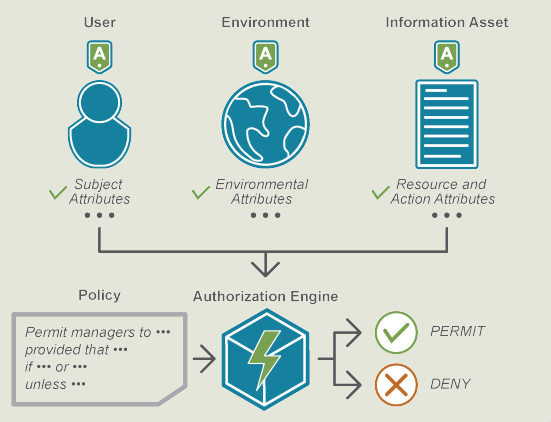
\includegraphics[width=\linewidth]{02P/ABAC.png}
        \caption{ABAC.}
        \label{fig:abac}
    \end{minipage}
    \hfill
    \begin{minipage}{0.45\textwidth}
        \centering
        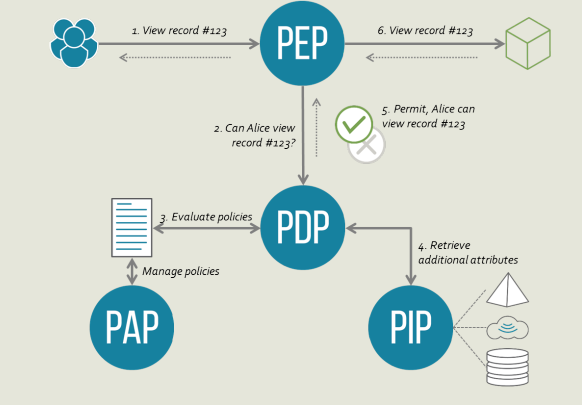
\includegraphics[width=\linewidth]{02P/engine.png}
        \caption{Dettaglio dell'authorization engine.}
        \label{fig:auth}
    \end{minipage}
\end{figure}

\nt{Le policies sono espresse in XACML (eXtensible Access Control Markup Language).}

\section{Pseudoanonimizzazione con Crittografia}

\dfn{Pseudoanonimizzazione}{
  La pseudoanonimizzazione è una procedura di data management e di deidentificazione per cui informazioni identificabili in un record sono rimpiazzate da uno o più identificatori artificiali (pseudonimi).
}

\nt{Un singolo pseudonimo viene utilizzato in modo consistente per permettere un'analisi accurata. Tuttavia questi dati pseudoanonimizzati possono essere riportati al loro stato originale perché viene salvata l'associazione con lo pseudonimo.}

\cor{Crittografia su Colonne}{
  La Crittografia su colonne è una feature per proteggere dati sensibili nei databases. Permette di crittografare dati sensibili senza rivelare la chiave all'engine del database. Questo fornisce una separazione tra:

  \begin{itemize}
    \item Chi possiede i dati e può visualizzarli. 
    \item Chi gestisce i dati, ma non ha il diritto di accedervi.
  \end{itemize}
}

\paragraph{Ci sono due tipi di chiavi:}

\begin{itemize}
  \item \fancyglitter{Column encryption keys:} per crittografare il dato. 
  \item \fancyglitter{Column master keys:} per crittografare la column encryption key.
\end{itemize}

\nt{Le chiavi non sono mai memorizzate nei meta dati, ma vengono salvate in un repository esterno.}

\paragraph{Crittografia deterministica vs. randomizzata:}

\begin{itemize}
  \item \fancyglitter{Crittografia deterministica:} genera sempre gli stessi valori per ogni testo. 
  \item \fancyglitter{Crittografia randomizzata:} utilizza valori casuali. È più sicura, ma impedisce le ricerche sul database.
    
\end{itemize}

\paragraph{Rivest-Shamir-Adleman (RSA):}

\begin{itemize}
  \item È un sistema crittografico a chiave pubblica. 
  \item Gli utenti creano e pubblicano una chiave pubblica basata su due numeri primi sufficientemente grandi segreti.
  \item I messaggi possono essere crittati da chiunque usando la chiave pubblica. 
  \item Possono essere decrittati solo da chi conosce la chiave privata.
  \item Utilizza anche un sistema di padding.
\end{itemize}

\paragraph{TDE (Oracle):}

\begin{itemize}
  \item Si usa sempre una sola chiave di crittografia. 
  \item Nessuna chiave è salvata in chiaro. 
  \item Il repository esterno di Oracle è chiamato Oracle wallet. 
  \item Vengono separate le responsabilità per prevenire accessi illeciti.
\end{itemize}

\subsection{Tracciabilità}









